\section{Generación de Lenguaje Natural}\label{s:nlg}
Como se ha descrito y observado gracias a la tabla \ref{tab:dailymail}, el tráfico de correos electrónicos diarios continúa en constante crecimiento hasta llegar, al menos, a la gigantesca cifra de 376 mil millones enviados al día en todo el mundo. Esto se revierte en una gran cantidad de tiempo invertido para la redacción de todos estos mensajes que no se mandan de manera automática. Sin embargo, esta gran dedicación al e-mail lleva produciéndose desde hace más de una década, cuando no nos encontrábamos con cifras de tráfico tan elevadas. Según \cite{mckinsey}, de media los empleados invertían el 28\% de su tiempo semanal en la gestión del correo electrónico (como viene reflejado en la figura \ref{fig:e-mailwork}). Esto se traduce en más de once horas dedicadas única y exclusivamente a leer y contestar mensajes, enviando y recibiendo una media de 124 e-mails por día \citep{radicati2015email}. Por si estos datos no fueran suficientemente preocupantes, de cara a la productividad laboral y resolución eficiente de las tareas, según \cite{forbes} este problema se ha agravado en los últimos años por diversas causas (entre las que se encuentra la pandemia de la Covid-19). En definitiva, hoy en día podemos afirmar que tanto en el ámbito profesional como personal se invierte una gran cantidad de esfuerzo y tiempo para gestionar nuestra cuenta de e-mail, lo cual plantea un problema en el que vemos que, en lugar de ser una herramienta útil, se convierte en una responsabilidad más que debe llevarse al día y de la que no es posible desprenderse ya que la capacidad de mandar estos mensajes es imprescindible para llevar a cabo tareas del día a día. Pero, ¿y si fuera posible ahorrar todo este tiempo de escritura de correos electrónicos?

\begin{figure}[h]
	\centering%
	\centerline{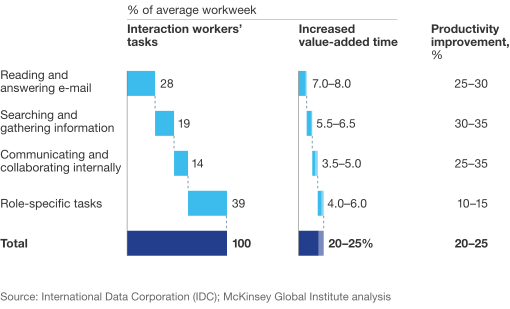
\includegraphics[width = 0.9\textwidth]{Imagenes/Bitmap/mckinsey.png}}%
	\caption{Porcentaje de tiempo de un trabajador dedicado a cada tarea}%
	\label{fig:e-mailwork}
\end{figure}

Para lograr este propósito es imprescindible profundizar en la rama de la Inteligencia Artificial conocida como \textit{Generación de Lenguaje Natural} (cuyas siglas son \textit{NLG} por su nombre en inglés \textit{Natural Language Generation}). Un buen ejemplo de aplicación de las técnicas de generación automática de textos son los 100.000 libros que Philip M. Parker puso a la venta en la plataforma \textit{Amazon.com} incluyendo títulos de temáticas tan variadas como \textit{El libro oficial del paciente sobre la estenosis espinal} \citep{parker2002official}, \textit{Perspectivas mundiales de 2009 a 2014 de los envases de 60 miligramos de Fromage Frais} \citep{parkerfromage},  \textit{Perspectivas de 2007 a 2012 de las tapetes de nudo, alfombras de baño y conjuntos que miden 6 pies por 9 pies o menos en la India} \citep{parkerrugs} y \textit{Tesauro Quechua - Inglés} \citep{parkerquechua}.

Resulta evidente que dicha cantidad de libros no pudieron ser escritos por Parker, sino que debió hacerse uso de técnicas de generación automática de textos. El algoritmo utilizado para dicho propósito, se engloba dentro de los métodos de generación conocidos como \textit{text-to-text} (texto a texto en castellano), dado que este tipo de técnicas toman como entrada textos ya existentes (normalmente escritos a mano y no generados automáticamente) y producen un nuevo texto coherente como salida. Otras aplicaciones de este tipo de métodos son la traducción automática de un idioma a otro \citep{hutchins2009introduction, oettinger2013automatic}, el resumen automático de textos \citep{mani2001automatic, nenkova2011automatic}, la simplificación de textos complejos, ya sea para hacerlos más accesibles para un público de lectores de bajo nivel de alfabetización \citep{siddharthan2014survey, bautista2011empirical} o niños \citep{macdonald2016summarising}, corrección automática de ortografía, gramática y texto \citep{kukich1992techniques, ng2014conll}, generación automática de revisiones de artículos científicos \citep{bartoli2016your}, generación de paráfrasis dada una frase de entrada \citep{bannard2005paraphrasing}, generación automática de preguntas con fines didácticos y educativos \citep{brown2005automatic}, generación automática de relatos dada una descripción conceptual de la historia deseada \citep{gervas2004story} o reescritura de textos (en concreto correos electrónicos) con estilo en función del destinatario \citep{mitfg}.

Además de estos métodos text-to-text, existen los llamados \textit{data-to-text} (datos a texto), en los cuales en lugar de recibir un texto como entrada, se genera el lenguaje a partir de datos. Estos pueden ser de todo tipo para dar lugar a informes o resúmenes como pueden ser de índole climatológica \citep{goldberg1994using, ramos2014linguistic}, financiera \citep{plachouras2016interacting}, ingenieril, como por ejemplo el trabajo desarrollado por \cite{yu2007choosing} para generar resúmenes de datos recopilados por sensores en turbinas de gas, sanitaria \citep{huske2003text, banaee2013towards}, como la investigación llevada a cabo por \cite{portet2009automatic} para obtener informes textuales a partir de datos de cuidados intensivos neonatales, o, incluso, deportivos \citep{theune2001data, chen2008learning}. Además de informes o resúmenes, también se utilizan los métodos \textit{data-to-text} para otros propósitos como la composición de discursos narrativos para relatos de varios personajes a partir de partidas de ajedrez \citep{gervas2014composing}, redacción de periódicos electrónicos a partir de datos de sensores \citep{molina2011generating}, generación de texto que aborda problemas medioambientales como el seguimiento de la fauna \citep{siddharthan2012blogging, ponnamperuma2013tag2blog}, la información medioambiental personalizada \citep{wanner2015getting} y la mejora del compromiso de los ciudadanos científicos a través de los comentarios generados \citep{van2016role} o producción de información interactiva sobre artefactos culturales \citep{stock2007adaptive}, entre otros.

Debido a que el objetivo de este trabajo se centra en la generación de correos electrónicos a partir del asunto, exploraremos en detalle las técnicas de Generación de Lenguaje Natural y, en especial, los métodos text-to-text. Para profundizar en los algoritmos y arquitecturas empleados ante los problemas de tipo data-to-text, conviene consultar la investigación llevada a cabo por \cite{gatt2018survey}, en la cual muestran el estado del arte de los trabajos realizados en este ámbito.

\subsection{¿Qué es la Generación de Lenguaje Natural?}
Dado que tanto los sistemas text-to-text como data-to-text y todas sus aplicaciones mencionadas anteriormente pertenecen a la rama de Generación de Lenguaje Natural, esta no debe definirse en función de la entrada del sistema, sino en la salida. Según \cite{biblia} la NLG es la conceptualización del ``campo de la inteligencia artificial y la lingüística computacional que se centra en los sistemas informáticos que son capaces de producir textos comprensibles en inglés u otra lengua humana. [...] Como área de investigación, la NLG presenta una perspectiva única ante problemas fundamentales de la inteligencia artificial, la ciencia cognitiva y la interacción. Estos incluyen cuestiones como por ejemplo cómo deben ser representados y cómo debe razonarse con la lingüística y el dominio del conocimiento, qué significa que un texto esté correctamente redactado y cómo es la mejor forma de comunicar información entre las computadoras y los usuarios.'' Por lo tanto, la Generación de Lenguaje Natural se puede definir como el ámbito que engloba el estudio de la producción de lenguaje no artificial, así como el diseño e implementación de algoritmos y sistemas computacionales cuyo resultado debe ser un texto que imite la forma en que los humanos se comunican verbalmente \citep{vicente2015generacion}, ya sea oralmente o por escrito \citep{del2007que}. Es decir, independientemente de la entrada recibida, se precisa el significado de NLG a partir de la salida esperada por el problema planteado. Tanto es así, que, como hemos visto, la entrada del sistema puede variar excesivamente \citep{mcdonald1993issues}: desde textos (que son precisamente los sistemas text-to-text) hasta datos de todo tipo como partidas de ajedrez \citep{gervas2014composing}, pictogramas \citep{gonzalez2019traductor} e, incluso, vídeos \citep{thomason2014integrating}. Sin embargo, autores como \cite{duvsek2020evaluating} acotan la definición de los sistemas de NLG estableciendo que la entrada deben ser representaciones semánticas, obviando así la primera tarea de la arquitectura propuesta por \cite{biblia} conocida como macro planificación o determinación del contenido (se explicará en la sección \ref{sss:realizer}), que es precisamente el punto en el que se generan dichas representaciones semánticas.

Cabe destacar que, aunque desde un principio hayamos diferenciado entre métodos text-to-text y data-to-text, ni los límites entre las dos aproximaciones ni la pertenencia de algunas técnicas a ellas se encuentran claramente definidos. Un ejemplo de ello podemos encontrarlo en la generación automática de resúmenes de textos. En principio se caracterizaría claramente como un sistema text-to-text. No obstante, al hacer frente a este problema se han desarrollado soluciones con las conocidas técnicas abstractivas \citep{genest2011framework}, que, como explican \cite{hahn2000challenges}, a diferencia de los métodos de extracción evitan recoger las frases completas y se limitan a tomar unidades semánticas. Este tipo de técnicas usadas, por ejemplo, en la obtención de opiniones de reseñas para la posterior generación de frases nuevas \citep{labbe2012towards}, también provienen de problemas data-to-text. A la inversa, un sistema data-to-text puede hacer uso de técnicas que principalmente son utilizadas en los casos de uso text-to-text \citep{mcintyre2009learning, kondadadi2013statistical}. Por otro lado, podría parecer que los métodos de \textit{deep learning} \citep{goodfellow2016deep} deben ser mayoritariamente utilizados en los problemas data-to-text utilizando el trabajo llevado a cabo por \cite{mikolov2013efficient}. Sin embargo, se han desarrollado extensamente esta clase de soluciones para la NLG con gran variedad de arquitecturas como las redes neuronales recurrentes \citep{cho2014learning, tang2016context}, muy a menudo combinadas con la memoria a corto plazo o LSTM \citep{chen2016enhanced}, o las arquitecturas conocidas como \textit{transformers} \citep{transformers}.

\subsection{Arquitecturas para la Generación de Lenguaje Natural}
Ante el problema de generación de lenguaje natural, se han propuesta diversas soluciones para abordarlo. Sin embargo, actualmente preponderan dos tipos de arquitecturas: la propuesta por \cite{biblia}, también conocida como arquitectura \textit{realizer} (toma el nombre de una de sus fases), que divide la generación en distintas subtareas y las aborda por separado, y la presentada por \cite{transformers}, también conocida como arquitectura \textit{transformer}, que expone una arquitectura constituida mayoritariamente por redes neuronales. Aunque en este trabajo hayamos hecho uso de esta última debido a la dificultad de establecer un dominio de lenguaje en los correos electrónicos, a continuación se hará una breve introducción a ambas.

\subsubsection{Arquitectura realizer}\label{sss:realizer}
A pesar de que en el trabajo de \cite{biblia} se centren principalmente en los sistemas de generación de lenguaje natural de tipo \textit{data-to-text}, esta arquitectura también ha sido utilizada por sistemas \textit{text-to-text} como para la generación automática de resúmenes a través de métodos abstractivos \citep{genest2011framework}. De hecho, incluso es posible hacer uso de la conceptualización de la entrada del sistema planteada por \cite{biblia} para este tipo de problemas.

La filosofía de esta arquitectura se centra en la modularización de las diferentes tareas a abordar durante la generación de lenguaje natural. De esta manera, cada módulo se enfrenta a un reto específico con el que debe lidiar y se conecta con el módulo anterior haciendo coincidir la salida del previo con la entrada del actual y, lo mismo, con el módulo posterior. Asimismo, se construye un \textit{pipeline} o arquitectura en secuencia de tareas con cada uno de los módulos.

La entrada de esta arquitectura viene determinada por una tupla de cuatro elementos $(k, c, u, d)$ donde cada uno de ellos puede representarse de distintas maneras. El primer elemento de la tupla es la \textit{base de conocimiento} (la letra viene dada por su denominación ingles \textit{knowledge source}). Se trata de la información acerca del dominio de nuestro sistema de generación de lenguaje natural, la cual suele consistir en un conjunto de bases de datos y bases de conocimiento, como las ontologías \citep{fensel2001ontologies}, que nuestra aplicación puede consultar durante su ejecución. Tanto la representación como el contenido de la base de conocimiento son altamente dependientes del tipo de aplicación que queramos construir, por ejemplo, en el trabajo de \cite{reiter2005choosing} la base de conocimiento consiste en parámetros meteorológicos numéricos de un modelo de predicción NWP, mientras que en el desarrollo presentado por \cite{reiter1995automatic} se utiliza como base de conocimiento un sistema de representación de conocimiento del mismo tipo que KL-ONE \citep{brachman1989overview} estructurado de manera jerárquica mediante relaciones \textit{is-a} y \textit{part-of}, del cual se pueden extraer diversas propiedades de las entidades que lo componen. Precisamente esta gran variabilidad en tan solo la primera componente de la entrada de la arquitectura realizer, es lo que sustenta la afirmación de \cite{biblia} de que no es posible proporcionar una caracterización formal genérica de lo que es una base de conocimiento y dificulta el establecimiento de esta componente en el sistema desarrollado si se hubiera elegido esta opción de arquitectura, ya que los correos electrónicos versan de una amplia variedad de temáticas muy distintas.

La segunda componente de la tupla de entrada es el objetivo de la comunicación (en inglés \textit{communicative goal}). Este describe el propósito del texto para el que se quiere generarlo. Es importante no confundirlo con el propósito general del sistema de generación de lenguaje natural. Por ejemplo, el objetivo final de sistema implementado por \cite{turner2007selecting} es generar resúmenes textuales de datos de predicción meteorológica numérica espacio-temporal. Sin embargo, su propósito comunicativo de una ejecución determinada es el de presentar predicciones meteorológicas de una localización geográfica y un momento temporal dados.

La letra u de la tupla se corresponde con el modelo de usuario (en inglés \textit{user model}), el cual consiste en una caracterización del receptor o público objetivo al que va dirigido el texto generado. Al igual que con el propósito comunicativo, no debe confundirse con los espectadores del sistema. Por ejemplo, el sistema implementado por \cite{reiter1999types} tiene como objetivo dirigirse a personas que consumen tabaco, ya que trata de generar cartas que convenzan a los pacientes con este hábito para que intenten superar su adicción. No obstante, no resulta adecuado utilizar el mismo tipo de técnicas de convicción y el mismo lenguaje para una persona que ha comenzado a fumar desde hace poco que a otra que lleva muchos años consumiendo tabaco. También, podría resultar interesante definir perfiles en función de la edad y otras características del paciente que permitirían personalizar aún más estas cartas. Son precisamente este tipo de propiedades las que englobaría el modelo de usuario que el sistema toma como entrada. No obstante, a pesar de que no existen demasiados ejemplos de trabajos que incluyan esta variable de entrada como lo desarrollan en su estudio \cite{goldberg1994fog}, por la dificultad de variación de los textos en función de dichos perfiles, este problema se suele tratar de abordar a través del estudio de la estilometría \citep{mitfg}.

El último componente de la entrada es la historia del discurso (en inglés \textit{discourse history}), la cual consiste en un modelo de la información transmitida y los temas tratados en el texto producido hasta el momento de la ejecución del sistema. Esto permite a la aplicación conocer las entidades y propiedades ya mencionadas gracias a las cuales es posible hacer un uso adecuado de los recursos anafóricos como los pronombres. En los sistemas de generación de lenguaje natural de interacción única, es decir, aquellos cuya ejecución produce un único texto con independencia de los generados en ejecuciones previas, la historia discursiva comienza como una estructura de datos vacía y se construye y utiliza durante la redacción del texto a generar. Todo lo contrario son los sistemas de diálogo, como los \textit{chatbots}, en los cuales la historia del discurso suele hacer referencia al registro de diálogo, utilizado como repositorio de información sobre las interacciones previas entre el usuario y la aplicación de NLG. En trabajos como el desarrollado por \cite{milosavljevic1996text}, en el cual se espera que los usuarios interactúen con una serie de textos relacionados, la historia discursiva resulta ser una mezcla de la utilizada en los sistemas de interacción única con la preponderante en los sistemas de diálogo. De esta manera, esta última componente de la tupla de entrada facilita el hacer referencias en el nuevo texto a entidades o conceptos mencionados en el texto actual o previos, o utilizar marcadores discursivos como ``como se ha mencionado anteriormente'' en momentos en que el texto generado repite información ya presentada en los anteriores.

Aunque puede resultar obvio, es importante tener en cuenta que, en la mayoría de los casos, será necesario un preprocesado del texto o los datos de entrada (sobre todo si han de ser analizados e interpretados) para facilitar el trabajo a la arquitectura presentada por \cite{biblia}, de manera que sea más sencillo utilizar la entrada en cada una de las fases \citep{han2011data}. Este primer preprocesado es plenamente opcional y depende del origen de la entrada que se vaya a utilizar.

Una vez se conoce la entrada y salida establecida para un sistema de generación de lenguaje natural, se puede comenzar la presentación de la arquitectura modular secuencial. Según \cite{biblia}, el proceso de generación puede descomponerse en tres fases: la macro planificación, la micro planificación y la realización (que da nombre a la arquitectura por ser la última fase). Los módulos que implementan cada una de ellas se conectan entre sí como muestra la figura \ref{fig:pipelinenlg}.

\begin{figure}[h]
	\centering%
	\centerline{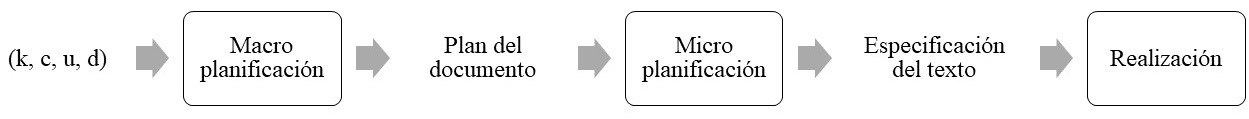
\includegraphics[width = \textwidth]{Imagenes/Bitmap/pipeline-nlg.jpg}}%
	\caption{Arquitectura modular secuencial propuesta por \cite{biblia} para la NLG}%
	\label{fig:pipelinenlg}
\end{figure}

En términos generales, el trabajo del módulo de macro planificación es producir una especificación del contenido del texto y su estructura, mediante el uso del dominio y el conocimiento de la aplicación sobre qué información es la más adecuada teniendo en cuenta la tupla de entrada. Esta fase normalmente también requiere conocer cómo suelen estructurarse los documentos del dominio de nuestro sistema. Muchas de las técnicas empleadas para la implementación de la macro planificación suelen asemejarse a las utilizadas en el ámbito de los sistemas expertos.

Para que el texto sea coherente, es preciso estructurar el contenido del mismo en el orden correcto. Por este motivo, la salida del módulo de macro planificación, el plan del documento, suele implementarse como una estructura de datos, generalmente arbórea, donde en cada nodo se encapsula la información más importante que debe formar parte de un párrafo o frase, además de información de cómo se relaciona con el resto de nodos. Con el objetivo de generar esta salida, se dividen las tareas de este nodo en determinación del contenido y estructuración del documento.

La determinación del contenido es la primera tarea de la macro planificación y, por tanto, del proceso de generación. En ella el sistema decide qué información es relevante para ser incluida en el texto y cuál no. Por lo general, en los sistemas data-to-text, se puede extraer más información en los datos de la que se quiere transmitir y, por ese motivo, cobra importancia la capacidad de selección y existen numerosas investigaciones al respecto, como la de \cite{yu2007choosing}. Aunque la determinación del contenido está presente en la mayoría de los sistemas de generación de lenguaje natural \citep{mellish2006reference}, los enfoques suelen estar estrechamente relacionados con el dominio, de forma que se construye una estructura de datos ad hoc,  denominada ``mensajes'', con el fin de especificar la salida de esta tarea (un ejemplo conceptual de un mensaje para un sistema que genera textos sobre la situación meteorológica puede observarse en la figura \ref{fig:messagenlg}). Este planteamiento de la determinación del contenido, dificulta el desarrollo de sistemas en los que el dominio es extenso, como es el caso de los correos electrónicos, ya que no es posible implementar una clase que englobe todas las casuísticas (como se verá en la sección \textcolor{red}{poner nº}, para resolver este problema se utilizará el concepto de \textit{Information Items} el cual pertenece al ámbito del resumen automático de textos). Sin embargo, sí se ha tratado de encontrar otro tipo de definición a la salida de esta tarea, como ocurre en el trabajo de \cite{guhe2007incremental}, el cual presenta una explicación cognitivamente plausible e incremental de la determinación del contenido, basada en estudios sobre las descripciones de observadores de eventos dinámicos a medida que se desarrollan.

\begin{figure}[h]
	\centering%
	\centerline{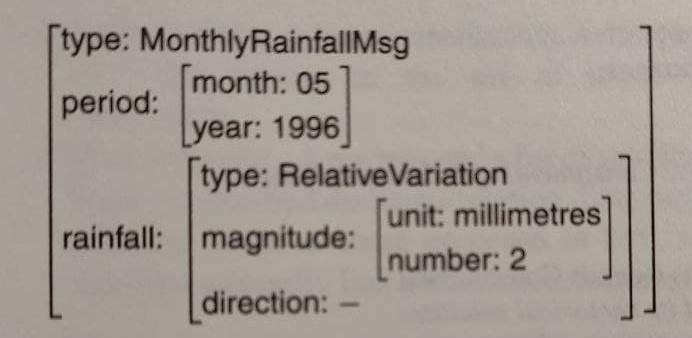
\includegraphics[width = 0.7\textwidth]{Imagenes/Bitmap/message-nlg.jpg}}%
	\caption{Ejemplo de mensaje}%
	Imagen extraída de \cite{biblia}
	\label{fig:messagenlg}
\end{figure}

La elección del contenido que debe ser expresado en el texto depende de varios factores, entre los que se encuentran: el propósito comunicativo, el modelo de usuario, las restricciones de la salida por limitaciones del dominio (como la longitud máxima que debe tener un texto) y la fuente de información (o base de conocimiento) subyacente disponible (es importante, aunque parezca evidente, no pretender generar información sobre la que el sistema no posee conocimiento o no es capaz de deducirlo con sus módulos de razonamiento correspondientes).
